\section{The artefact: Data Analysis as a Service (DAaaS)}
This section describes the design and implementation of Data Analysis as a Service (DAaaS), an artefact developed by Andreas Biørn-Hansen and Martin Lehmann as a prototype project prior to the writing of this article.

A clear gap identified in the previous section is the lack of of sample implementations of full-stack applications where communication, storage, analysis opportunities, and availability are all thoroughly discussed and actually implemented. DSaaS is an attempt to start bridging this gap, but will naturally only provide the perspective of one domain, one technology stack, and one use case.

Very briefly, DSaaS accepts and stores data from providers (sensors), pushes the new data to a very simple customisable dashboard (see \ref{fig:simple-dashboard}, and provides (optionally real-time) access to the data sets. Security is not considered in the prototype. It was implemented with the sole goal of building a complete application designed to handle data from the Internet and Web of things.

\begin{figure}[H]
    \label{fig:simple-dashboard}
    \centerline{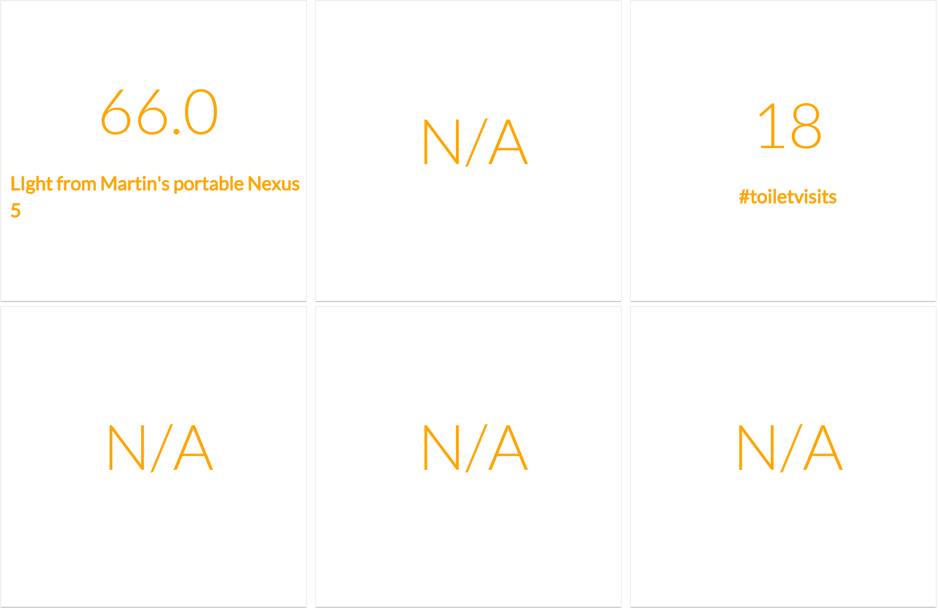
\includegraphics[scale=0.3]{dashboard-simple}}
    \caption{The simple dashboard with two integrations}
\end{figure}

The DSaaS core is a central server written in Meteor\footnote{\url{https://www.meteor.com/}} providing access to both storing and retrieving data. It also provides the option of subscribing to a changefeed for a specific resource to receive updates to the dataset in real-time. DSaaS also provides a very simple real-time dashboard for monitoring incoming data. Finally, it provides a management interface for customising the dashboard and defining the \textit{integrations} that can be displayed in the dashboard.

\begin{figure}[H]
    \label{fig:sample-integrations}
    \centerline{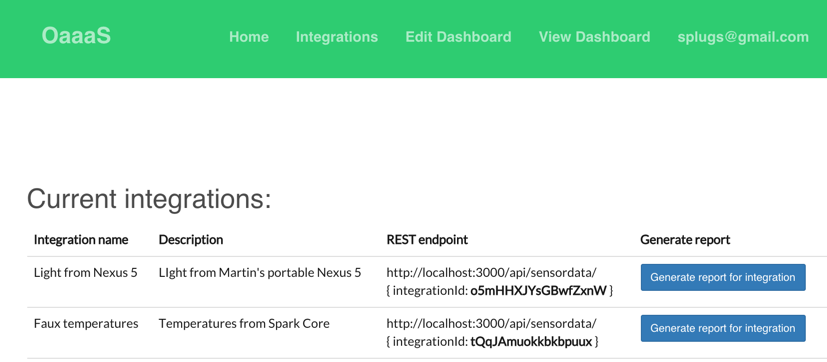
\includegraphics[scale=0.5]{sample-integrations}}
    \caption{Sample integrations}
\end{figure}

An \textit{integration} is a data provider of any kind that will upload data to the service. An integration is expected to be a single sensor whose data is sent to the internet - typically via an internet-enabled microcontroller -- although it is possible to get creative. As seen in \ref{fig:sample-integrations}, creating an integration automatically generates a unique ID, which must be included in requests to upload data as identification.

In addition to endpoints for storing data, DSaaS provides two different types of endpoints for accessing the stored data. The simplest of these is a traditional REST endpoint that exposes data from each sensor as a resource with a unique URI: an HTTP GET request fetches data from the present day. Of course, applying filters to fetch for example all stored data, data from the present week, or data from the last ten days, would be helpful -- but this was outside the scope of the prototype.

The second data access endpoint provides a real-time changefeed that sends all new relevant data points to the consumer as it is stored in the database. The protocol for real-time data updates is Meteor's Distributed Data Protocol (DDP), which is based on WebSockets. It would naturally be possible to define a custom protocol with plain WebSockets. This enables building real-time graphs or custom dashboards for the data, or real-time analysis with for instance Apache Storm\footnote{\url{https://storm.apache.org/}}.

The prototype also includes three sample integrations/data providers (a Spark Core microcontroller\footnote{\url{https://store.spark.io/?product=spark-core}}, a native Android application listening for light values in the room using the light sensor on the mobile device, and a simple Ionic\footnote{\url{http://ionicframework.com/}} cross-platform application for mobile and web for registering a single value.

Finally, the prototype includes one external real-time consumer written in JavaScript, which is a proof-of-concept realtime graph for a single sensor. 
